\documentclass[main.tex]{subfiles}

\begin{document}

\section{Условие задачи}

\subsection{Законы Кирхгофа для перераспределения потоков между трещинами}

Весь расход, который закачиваем в скважину, перераспределяется между трещинами (первый закон Кирхгофа):
\beq
Q_0=\sum_{i=1}^{N}{Q_i}
\eeq

Можно независимо рассматривать каждый из путей (к каждой из трещин) и считать гидродинамические сопротивления независимо (второй закон Кирхгофа):
\beq
p_0=\sigma_{min,i}+p_{net,i}+\Delta p_{perf,i}-\sum_{j=1}^{i}{\Delta p_{h,j}}+\sum_{j=1}^{i}\Delta p_{fric,j},
\eeq
где

$\sigma_{min,i}$ -- давление закрытия (минимальное напряжение в пласте) на $i$-ой трещине;

$p_{net,i}=p_{frac,i}-\sigma_{min,i}$ -- давление на $i$-ой трещине (из модели трещины);

$\Delta p_{perf,i}$ -- падение давления вдоль перфорации $i$-ой трещины;

$\Delta p_{h,i}$ -- падение гидростатического давления между $i$-ой и $(i-1)$-ой трещинами;

$\Delta p_{fric,i}$ -- падение давления на трение между $i$-ой и $(i-1)$-ой трещинами.
\\

В итоге, получаем следующую систему уравнений:
\beq
\begin{cases}
Q_0=\sum\limits_{i=1}^{N}{Q_i}\\
p_0=\sigma_{min,i}+p_{net,i}(Q_i)+\Delta p_{perf,i}(Q_i)-\sum\limits_{j=1}^{i}{\Delta p_{h,j}}+\sum\limits_{j=1}^{i}\Delta p_{fric,j}(Q_i)
\end{cases}
\eeq
относительно неизвестных расходов $Q_i$ и забойного давления $p_0$.


\subsection{Формула для давления $p_{net,i}$ на $i$-ой трещине}

Аналитический подход (с использованием PKN модели):
\beq
p_{net,i}(Q_i)=a_iQ_i^{\frac{n}{2n+3}}V_i^{\frac{1}{2n+3}},
\eeq
где $a_i=\left(\dfrac{(n+3)(2n+1)^n \cdot K\cdot (E_i')^{2n+2}}{\pi\, 2^{2n}n^n\phi^n h_i^{3n+3}}\right)^{\!\frac{1}{2n+3}}$ -- параметр жёсткости,
\\

$Q_i$ и $V_i$ -- расход на $i$-ой трещине и объём $i$-ой трещины;

$K$ и $n$ -- реологические параметры степенной (неньютоновской) жидкости;

$E_i'$ -- модуль плоской деформации $i$-ой трещины;

$h_i$ -- мощность продуктивной зоны.


\subsection{Формула для падения давления $\text{Δ} p_{perf,i}$ на перфорациях}

Эмпирическая формула для падения давления на перфорациях:
\beq
\Delta p_{perf,i}=\frac{8\rho_s}{\pi^2 C_{d,i}^2 n_{p,i}^2 d_{p_i}^4}Q_i\left|Q_i\right|,
\eeq
где $\rho_s$ -- средняя плотность смеси;

$n_{p,i}, d_{p,i}$ -- количество и диаметр перфораций;
\\

$C_{d,i}=\dfrac{\text{min}(d_{jet})}{d_p}$ -- безразмерный коэффициент эррозии (в случае отсутствия твёрдых частичек в потоке $C_{d,i}\in\left[0.5,0.6\right]$, а с твёрдыми частичками в потоке $C_{d,j}\in\left[0.6,0.95\right]$  из-за эррозии перфорации).

\subsection{Формула для гидростатического давления $\text{Δ} p_{h,i}$}

Гидростатическое давление на каждом интервале рассчитывается по следующей формуле:
\beq
\Delta p_{h,i}(t,x)=\int\limits_{x_{i-1}}^{x_i}{\rho(c(t,s))\cdot g\cdot \sin{(\theta(s))}ds},
\eeq
где $x_i$ -- измеренная глубина (MD) $i$-ой трещины;

$\rho(c(t,s))$ -- плотность смеси, которая зависит от динамически меняющейся концентрации проппанта;

$g$ -- ускорение свободного падения;

$\theta(s)$ -- угол между скважиной и поверхностью Земли в данной точке.

\subsection{Формула для падения давления $\text{Δ} p_{fric,i}$ на трение}

Падение давления на трение на каждом интервале рассчитывается по следующей формуле:
\beq
\Delta p_{fric,i}=\int\limits_{x_{i-1}}^{x_i}{f\frac{\rho u_{m,i}^2}{R_i}}=\int\limits_{x_{i-1}}^{x_i}{\frac{\rho(c(t,s))\cdot f(Re)\cdot \left(Q_0-\sum\limits_{j=1}^{i-1}{Q_j}\right)^{\!2}}{R_i(s)S_i^2(s)}}ds,
\eeq
где $f=\dfrac{\tau}{\rho u_{m,i}^2/2}$ -- коэффициент трения Фаннинга;

$\rho(c(t,s))$ -- плотность смеси, которая зависит от динамически меняющейся концентрации проппанта;

$u_{m,i}=\dfrac{Q_0-\sum\limits_{j=1}^{i-1}{Q_j}}{S_i}$ -- средняя скорость на рассматриваемом участке трубы;

$S_i$ -- площадь сечения рассматриваемого участка трубы;

$R_i$ -- радиус рассматриваемого участка трубы;

$Re$ -- число Рейнольдса.

\subsection{Итеративная процедура решения с помощью метода Ньютона}

\includegraphics[width=\textwidth, page=91]{HF_slides_2022.pdf}

\includegraphics[width=\textwidth, page=92]{HF_slides_2022.pdf}


\end{document}
